\documentclass[11pt,twoside,a4paper]{report}


% ------- Enable UTF8 characters ------- %
\usepackage[utf8]{inputenc}
\usepackage[english]{babel}


% --------------- Math ----------------- %
\usepackage{amsmath}
\usepackage{amsfonts}
\usepackage{mdframed}
\newcommand{\dif}{\mbox{$\mathrm{d}$}}
\newcommand{\ohm}{\mbox{$\Omega$}}

% ------------- Figures & Tables -------------- %
\usepackage{graphicx}
\usepackage{caption}
\usepackage{float}
\usepackage{subcaption}
\captionsetup[figure]{singlelinecheck=false, margin=0pt,labelsep=space,labelfont=bf,textfont=it}
\captionsetup[table]{singlelinecheck=false, margin=0pt,labelsep=space,labelfont=bf,textfont=it}
\usepackage{epstopdf} %MATLAB eps (vector) figures

\usepackage{array}
\newcolumntype{x}[1]{>{\centering\let\newline\\\arraybackslash\hspace{0pt}}p{#1}}


% --------------- Color ---------------- %
\usepackage{color}
\definecolor{dkgreen}{rgb}{0,0.6,0}
\definecolor{gray}{rgb}{0.5,0.5,0.5}
\definecolor{mauve}{rgb}{0.58,0,0.82}


% --------------- Code ----------------- %
\usepackage{verbatim}
\usepackage{listings}
\lstset{
	frame				= lines,
  	language				= C++,
  	aboveskip			= 3mm,
  	belowskip			= 3mm,
  	captionpos			= t,
  	showstringspaces		= false,
  	columns				= flexible,
  	basicstyle			= {\small\ttfamily},
  	numbers				= left,
  	numberstyle			= \tiny\color{gray},
  	keywordstyle			= \color{blue},
  	commentstyle			= \color{dkgreen},
  	stringstyle			= \color{dkgreen},
  	breaklines			= true,
  	breakatwhitespace	= true,
  	tabsize				= 3,
  	xleftmargin			= 17pt,
  	framexleftmargin		= 17pt,
  	framexrightmargin	= 17pt,
  	framexbottommargin	= 5pt,
	framextopmargin		= 5pt,
	moredelim			= **[is][\color{mauve}]{@}{@}
}
\lstset{
	literate				= {~} {\raise.17ex\hbox{$\scriptstyle\sim$}}{1}
}


\lstdefinelanguage{pseudo}{
  sensitive=false,
  morecomment=[l]//
}
\lstdefinestyle{pseudo}{
  language     = pseudo,
  commentstyle = \color{dkgreen}
}



\DeclareCaptionFormat{listing}{\rule{\dimexpr\textwidth+17pt\relax}{0.4pt}\par\vskip1pt#1#2#3}
\captionsetup[lstlisting]{format=listing,singlelinecheck=false, margin=0pt,labelsep=space,labelfont=bf}

\renewcommand\lstlistingname{Listing}



% ----------- Page Layout ------------- %
\usepackage{fullpage}
\headsep = 24pt % spacing between header and text
\usepackage{fancyhdr}
\usepackage{lastpage}
\usepackage{paralist}
\fancyhf{}
\fancyhead[LE]{\slshape \rightmark} % section
\fancyhead[RE]{\thepage}
\fancyhead[RO]{\slshape \leftmark} % chapter
\fancyhead[LO]{\thepage}
\pagestyle{fancy}
\setlength{\headheight}{15pt}


% font
\usepackage[T1]{fontenc}

\usepackage{titlesec}
\titleformat{\chapter}[display]
{\normalfont\Large\filleft}
{\sc\chaptertitlename\ \Huge{\thechapter}\\%
\vspace{1.5cm}
\titlerule[1pt]}
{-20pt}
{\Large}[\vspace{2ex}{\titlerule[1pt]}]

\titleformat{name=\chapter,numberless}[display]
{\normalfont\Large\filleft}
{}
{0pt}
{\titlerule[1pt]
\vspace{2ex}%
\Large}[\vspace{2ex}{\titlerule[1pt]}]

\titlespacing*{\chapter} {0pt}{0pt}{40pt}   %% adjust these numbers
\titlespacing*{name=\chapter,numberless} {0pt}{0pt}{40pt}   %% adjust these numbers


\newcommand{\HRule}{\rule{\linewidth}{0.3mm}}
\usepackage{blindtext} %Lorem Ipsum replica

% -------- Table of Contents --------- %
\usepackage[titles]{tocloft}
\usepackage[toc,page]{appendix}
\setlength{\cftbeforesecskip}{0pt}
\setlength{\cftbeforechapskip}{7pt}
\setlength{\cftbeforetoctitleskip}{-20pt}



% -------- TikZ --------- %
\usepackage{tikz}
\usepackage{circuitikz}
\usepackage{tikz-timing}
%\input{timing}
\usepackage{pgf}
\usetikzlibrary{arrows,automata}
\usetikzlibrary{patterns}
\usetikzlibrary{shapes.geometric}

\usetikzlibrary{fit}
\usetikzlibrary{calc}
\usetikzlibrary{intersections}
\usetikzlibrary{backgrounds}

\tikzset{desc/.style={outer sep=0pt,inner sep=0pt,text centered,font=\scriptsize,fill=black!10}}

\newcommand{\texta}{Helpful\\ \tiny (to achieve the objective)}
\newcommand{\textb}{Harmful\\ \tiny (to achieve the objective)}
\newcommand{\textc}{\rotatebox[origin=r]{90}{\shortstack{Internal origin\\ \tiny (product\slash company attributes)}}}
\newcommand{\textd}{\rotatebox[origin=r]{90}{\shortstack{External origin\\ \tiny (environment\slash market attributes)}}}


% -------- To Do notes --------- %
\usepackage{todonotes}


%---------- URL ----------%
\usepackage{hyperref} % clickable references
\hypersetup{
    colorlinks,
    citecolor=black,
    filecolor=black,
    linkcolor=black,
    urlcolor=blue,
    pdfborder = { 0 0 0 }
}
\def\UrlFont{}

%\usepackage[numbers, square, comma, sort&compress]{natbib}

\usepackage[
  backend=bibtex,
  %style=alpabethical,
  citestyle=verbose%-tcomp
  ]{biblatex}
\bibliography{bibliography} 

\usepackage[hang,flushmargin]{footmisc}


\begin{document}

% --------- Title Page, Front Page --------- %
\setcounter{page}{1}
\pagenumbering{Alph}

\begin{titlepage}

%\newcommand{\HRule}{\rule{\linewidth}{0.5mm}} % Defines a new command for the horizontal lines, change thickness here

\center % Center everything on the page
 


%----------------------------------------------------------------------------------------
%	TITLE SECTION
%----------------------------------------------------------------------------------------

\HRule \\[0.4cm]
{ \huge \textbf{ Controlling multiple drones autonomously \\ inspired by birds ability to keep formation}}\\[0.4cm] % Title of your document

\HRule \\[1.5cm]
\includegraphics[width=0.4\textwidth]{University_of_Southern_Denmark-logo} \\
\textsc{\large \emph{University:} \\   University of Southern Denmark }\\[0.5cm] % Major heading such as course name
\textsc{\large \emph{Author:} \\ Mathias Mikkel Neerup }\\[0.5cm] % Minor heading such as course title

%----------------------------------------------------------------------------------------
%	HEADING SECTIONS
%----------------------------------------------------------------------------------------

\LARGE Bachelor Thesis\\[1.5cm] % Name of your university/college
 
%----------------------------------------------------------------------------------------
%	AUTHOR SECTION
%----------------------------------------------------------------------------------------

\begin{minipage}{0.4\textwidth}
\begin{flushleft} \large
\emph{In coorperation with:}\\
Jussi Hermansen \\
Info@viacopter.eu \\
Cottagevej 4  \\
3300 Frederiksvaerk \\
\end{flushleft}
\end{minipage}
~
\begin{minipage}{0.4\textwidth}
\begin{flushright} \large
\emph{Supervisor:} \\
Kjeld Jensen \\ % Supervisor's Name
kjen@mmmi.sdu.dk \\
Maersk Mc-Kinney Moeller \\
University of Southern Denmark
\end{flushright}
\end{minipage}\\[4cm]


% If you don't want a supervisor, uncomment the two lines below and remove the section above
%\Large \emph{Author:}\\
%John \textsc{Smith}\\[3cm] % Your name

%----------------------------------------------------------------------------------------
%	DATE SECTION
%----------------------------------------------------------------------------------------

{\large June 1, 2016}\\[3cm] % Date, change the \today to a set date if you want to be precise

%----------------------------------------------------------------------------------------
%	LOGO SECTION
%----------------------------------------------------------------------------------------

%\includegraphics{Logo}\\[1cm] % Include a department/university logo - this will require the graphicx package
 
%----------------------------------------------------------------------------------------

\vfill % Fill the rest of the page with whitespace

\Mathias{A bachelors thesis (15 ECTS) report from a single student should have a length no more than 35 
pages plus maximum 10 pages of appendices.}
\Mathias{Ja, men gør det som elektronisk bilag (pdf) og beskriv i rapporten, at den ligger der. Marker det evt. dine bidrag med farve, så det er meget let at se. }
\end{titlepage}

\input{titlepage}



% --------- Front Matter --------- %
\setcounter{page}{1} % Start counter at 1
\pagenumbering{roman}

\section*{Acknowledgement}
Throughout the project period my classmates has been at great help to discuss and generate ideas.

Especially thanks to the people listed below.
\begin{itemize}
	\item My supervisor Kjeld Jensen for giving solutions and help when needed.
	\item Developer of MarkerLocator Henrik Midtiby for helping me understand and adding functionality to his software.
	\item Friend Morten Albeck Nielsen for meeting once a week to help generating ideas, debugging, sparring and proof reading the thesis.
	\item Friends Mads Tilgaard Jensen, Eskild Andresen \& Michael René Andersen for listening to technical issues, evaluating solutions and carrying out tests.
	\item My girlfriend Anna Riisberg Soerensen for proofreading the thesis and understanding the time required throughout this project period.
\end{itemize}



\chapter*{Abstract}
\addcontentsline{toc}{chapter}{Abstract}
Until now drones keeps getting bigger and larger to carry bigger batteries with more capacity and to lift heavier payloads. This leads to drones getting less efficient, less responsive and gets more dangerous. Instead it has become popular to make drones smaller and increase the number of drones needed to solve a task. \\

(Materials \& methods) \\
This thesis describes how to make three drones follow a leader drone with a preprogrammed path as an example of drones cooperating. A Linux PC running MarkerLocator tracks each drones position and wirelessly transmits, using Xbee, the drones positions to all drones.The position of each drone is spoofed into the drone using the CAN-bus and thereby overwriting the onboard GPS. An outdoor test has been made using the onboard GPS to test the leader-follower algorithm in a bigger scale. A small PCB has been developed and mounted on each drone to route packages from the Xbee module to the CAN-bus of the drone and to measure the local altitude of the drone using a ultrasonic sensor. The PCB carries an AT90CAN128 as microcontroller which build-in CAN support making it obsolete to carry an external USB CAN-controller.\\


(Results -> discussion)\\
The accuracy of the vision based localisation is measured using a laser pointer pointing out the drones 2D position on the floor making it possible to measure the variance of the drones position. The leader-follower algorithm was also tested outside using the onboard GPS. The performance of the leader-follower algorithm is measured and discussed using plots that reveals the distance between the drones.\\

(Conclusion -> perspective)\\
It is shown that it is possible to implement the leader-follower algorithm using a vision and ultrasonic based positioning system. The distance between all drones when flying indoor was +/- 10 cm which is less than the maximum accepted error. It was possible to add 5 follower-drones without editing the code showing it is a generic system The system can further be used to indoor testing of navigation algorithms and explore the many possibilities drones has to offer. If drones at some point needs to fly indoor to help eg. Mobile robots navigating, vision might be a way to obtain a absolute indoor position for the drones.

\chapter*{Reading Guide}
\addcontentsline{toc}{chapter}{Reading Guide}
This thesis contains three parts.\\ \\
\textbf{Chapter 1} gives background information about the purpose of this project. It starts giving an overview of the topic and ends up focusing on why it makes sense to make the project and what other universities have done. It further contains related work,  problem statement, defined hypothesis and assumptions and limitations. A image of the final extension board can be seen to make it clear to the reader how the developed extension board and AutoQuad Ladybird drone looks\\ \\
\textbf{Chapter 2} describes materials and methods used in this thesis. It explains how and why the following design chooses where made concerning firmware as well as developed PCB. Each chapter starts with an introduction and ends with test results evaluating weather the choices made works or not.\\ \\
\textbf{Chapter 3,4,5} concerns showing, analyzing and discussing results. Evaluation of the design choices made throughout chapter 2 with respect to the hypothesis is summarized in the conclusion. \\


On figure \ref{fig:drone_with_arrows} the different parts used in this thesis are highlighted.

\begin{figure}[H]
    \center
    \includegraphics[width=0.65\textwidth]{graphics/m4_arrow.png}
  \caption{Ladybird M4 drone with developed extension board}
  \label{fig:drone_with_arrows}
\end{figure}

\chapter*{Terms and Notation}
\addcontentsline{toc}{chapter}{Terms and Notation}
\input{terms_notations}

\newpage
\renewcommand\contentsname{Table of Contents}
\tableofcontents
%\addtocontents{toc}{\vskip-70pt}
\newpage




% --------- Main Matter --------- %
\setcounter{page}{1} % Start counter at 1
\pagenumbering{arabic}

\chapter{Introduction}\label{chp:Intro}
\textit{This chapter will give the reader background information about UAVs and point out a problem SDU is currently facing in two ongoing projects. Further more it will describe the focus of this project and how others have managed to solve it.}
\Mathias{Indøres navigation \url{http://innovationsfonden.dk/da/case/droner-rykker-indendoers-med-dansk-teknologi-0}}
\subsection*{Background}
UAS is an emerging technology\footcite{gupta2013review} used in lots of different areas. They are used in military purposes since UAVs are better suited for dull, dirty, or dangerous missions than manned aircraft. They are also widely used commercially to provide images of fields, power lines, pipelines \footnote{\url{https://en.wikipedia.org/wiki/Unmanned\_aerial\_vehicle\#Civil}} and so forth.\\
Since UAVs, especially multiroters or quadcopters, have become less expensive to produce, a marked for civilians and hobbyists has emerged. At the moment of writing, SDU is developing \footnote{\url{http://videnskab.dk/teknologi/droner-skal-have-elektronisk-nummerplade}} a registration plate, so that it is possible to see where drones are flying and who to be held responsible when accidents occur.

\textcolor{blue}{A challenge concerning multiroters and especially multiroters is the amount of energy they are capable of carrying. A drone designed with long flytime in mind is capable of flying approximately 20 minutes depending on weather and payload. If the drone is equipped with a heavy camera or other kind of payload, then the flight time begins to decrease rapidly. So far the solution has been to increase the size of the drones to mount bigger batteries, but this might not be right way of doing it. Drones become less efficient, less responsive and gets more dangerous due to increase in weight.\\
By looking at the nature, one can see how small animals like ants and birds manage to cooperate and thereby build or move bigger things that they would not be able to do on their own. This way of small independent, decentralized units working together is called a swarm\footnote{\url{https://en.wikipedia.org/wiki/Swarm\_intelligence}}.\\
By making UAVs smaller, they get more efficient, their flight time increase and they get cheaper but of the cost of their ability to lift\footcite{1_kumar_2016}. Therefore it seems like an idea to make small drones cooperate to solve more complex tasks.} \\

Many different flight pilots exists on the marked. SDU UAS has decided to use AutoQuad since the code is Open Source \footnote{Quatos, which is their control algorithm is not Open Source.} and the multiroters show reliable and steady flying. An AutoQuad multiroter delivered by ViaCopter\footnote{\url{https://viacopter.eu/}} comes with with the AutoQuad flight controller M4, Electronic Speed Controllers \footnote{Number depends of rotors on UAV} ESC32 and rotors. ViaCopter smallest drone is delivered without Electronic Speed Controllers since H-bridges are build into the M4 flight pilot.
ViaCopter delivers drones in different sizes but their flight controller is the same. This means that code developed for ViaCopters Ladybird can be deployed on a large drone and it will continue to work\footnote{Assumed the developer did not break important lowlevel tasks}

\begin{figure}[H]
    \centering
    \begin{subfigure}[b]{0.3\textwidth}
        \includegraphics[width=\textwidth]{graphics/M4_demo}
        \caption{M4 flight pilot}
        \label{fig:gull}
    \end{subfigure}
    ~ %add desired spacing between images, e. g. ~, \quad, \qquad, \hfill etc. 
      %(or a blank line to force the subfigure onto a new line)
    \begin{subfigure}[b]{0.3\textwidth}
        \includegraphics[width=\textwidth]{graphics/ladybird}
        \caption{Ladybird with mounted M4}
        \label{fig:tiger}
    \end{subfigure}
    ~ %add desired spacing between images, e. g. ~, \quad, \qquad, \hfill etc. 
    %(or a blank line to force the subfigure onto a new line)
    \begin{subfigure}[b]{0.3\textwidth}
        \includegraphics[width=\textwidth]{graphics/eduquad.jpg}
        \caption{Eduquad with M4 + ESC32}
        \label{fig:mouse}
    \end{subfigure}
    \caption{Pictures of AutoQuad hardware}\label{fig:AQ_hw}
\end{figure} 

At the time of writing, SDU is collaborating with HCA airport to find anomalies in fences.\\ 
\textit{Airports are burdened by a number of required inspection tasks to maintain a high level of 
safety and security.
Some of these tasks may advantageously be performed by a drone rather than the current manual labour, and this will save significant resources.
In this project they are targeting a specific need for frequent inspection of the fence surrounding the airport shown in figure \ref{fig:hca_fence}. 
The inspection concerns fence holes or similar anomalies. We hypothesize that a drone is 
capable of unsupervised autonomous inspecting the airport fence detecting small holes down 
to a radius of 5 cm.} \footnote{Application sent to Energi Fyns Udviklingsfond which has been granted, Ansøgning 2015-01-30 Energi Fyns Udviklingsfond-1.pdf on USB}

\begin{figure}[H]
    \centering
    %(or a blank line to force the subfigure onto a new line)
    \begin{subfigure}[b]{0.45\textwidth}
        \includegraphics[width=\textwidth]{graphics/hca_fence.png}
        \caption{Part of the fence surrounding HCA Airport.}
        \label{fig:hca_fence}
    \end{subfigure}
        ~  %add desired spacing between images, e. g. ~, \quad, \qquad, \hfill etc. 
    %(or a blank line to force the subfigure onto a new line)
    \begin{subfigure}[b]{0.45\textwidth}
        \includegraphics[width=\textwidth]{graphics/organicdrone.png}
        \caption{Drone spreading ladybirds and gall midges to avoid spreading pesticides in organic crops}
        \label{fig:organicdrone}
    \end{subfigure}
   \label{fig:sdu_projects}
\end{figure}
\Mathias{Huske at skrive hvem der støtter projekt samt med hvor meget de er støttet}
In order to avoid flying into the fence and to fly accurate enough for the camera to film, it is required to use an RTK GPS\footcite{2_gakstatter_2014}.

In another project, SDU is working together with a company, Ecobotix, to avoid the need of pesticides in organic crops. Pesticides are used to kill pests from the crows. When using pesticides a health risks exists for those who eat the crops. The use of pesticides also reduce the amount of diversity in nature since it is also killing beneficial organisms and potentially harm other animals in the food chain like birds. If nothing is used the crops might die, and that is very expensive to the farmer. \footnote{\url{http://naturerhverv.dk/tvaergaaende/gudp/gudp-projekter/2015/oekodrone-skal-sprede-mariehoens-i-stedet-for-pesticider/} last visited 18-04-2016}\\
SDU and Ecobix use drones to spread bugs like ladybirds and gall midges, over the crops to eat pests as shown in fugure \ref{fig:organicdrone}. \\
It is required the drones fly approximately 1 meter above ground at 1.5 meter/sec. It is therefore necessary to use an RTK-GPS in order to avoid hitting the ground in case of pumps in the fields. \footnote{Jensen, K.; Larsen, R.; Laursen M.S.; Neerup, M.M.; Skriver, M. and Jørgensen, R.N. Towards UAV contour flight over agricultural fields using RTK-GNSS and a Digital Height Model. Accepted for oral presentation at CIGR-AgEng June 2016.}\\
Both projects tends to use AutoQaud to solve their tasks. The AutoQuad version available at the moment of writing only supports autonomous flying using its onboard GPS. This project extends AutoQuads functionality by making it support global positioning from an RTK-GPS. 

\newpage
\subsection{Problem Statement}
The current AutoQuad does not support vision as source of 2D position which is required for the indoor Leader-follower to work. The relative height of the drone is measured using the build-in barometer in each drone providing the third dimension to the drones position. In case the barometer turns out to be too inaccurate due to drift other sensors might be used e.g ultrasound. The computer has to send waypoints wirelessly to all of the drones. A PCB for each drone has to be developed for the drones to carry as payload. The PCB will be responsible for receiving messages from the computer and translate them into the CAN-bus of the drone.
Hypothesis
If each drone’s 2D position is obtained using vision and spoofed into the drone using CAN, then it is possible for at least 3 drones to follow a leader drone with a preprogrammed flight path and keep a euclidean distance at 50 cm within plus minus 10 cm to the leader and its neighbours.

\subsection{Related Work}
In order to find relevant research about drones flying indoor, a few search phrases was conducted.
The following keywords were used to create different phases: Indoor, environment, swarm, localization, AutoQuad, quadrotor, mini UAV, test facilities, ETH, accurate, RTK, totalstation.
Based on the keywords a few papers was deemed relevant to the project and has been combined in order to give the reader an overview within the field of this project. \\

Developers of AutoQuad did previously try to implement RTKLib \footnote{http://www.rtklib.com} in AQ. Unfortunately they did manage to make it work as expected \footnote{Jussi Hermansen, owner of \url{http://ViaCopter.eu}}.\\

One of the big players within the field of indoor navigation and controlling multiple drones accurately is the university ETHzûrich and their Institute for Dynamic Systems and Modelling \footnote{\url{http://www.idsc.ethz.ch/research-dandrea/research-projects/aerial-construction.html}}. They have developed a test flying area they call "Flying Machine area" which provides facilities for doing prototype testing of new control algorithms \footcite{lupashin2014platform}. The FMAs dimensions is 10*10*10m and provides nets to protect people and mattresses to protect the drone  if a crash. The FMA has further been developed into a mobile installation to be used in demonstrations in Europe and North America. One of their demonstrations where used in a TED video about multiroters and their capabilities \footnote{https://www.ted.com/talks/raffaello\_d\_andrea\_the\_astounding\_athletic\_power\_of\_quadcopters}.
The multiroter usually used in the FMA is Ascending Technologies' Hummingbird with custom wireless communication and electronics. \\
They have build it as a module design in order to be easy to replace parts of their system by simulations and to make it scalable.
One of their modules is a copilot that implements an accident handler in case of user-code crashing or sending invalid commands to the drones.
They are using UDP multicast packets as communication between ground computation and flying objects. The use of UDP multicast packets between modules since to makes the system more simple but also to avoid the need of buffers to handle unsuccessful transmissions and retransmissions. \\
In order to detect the quadroters they are using a commercial motion capture system. Three reflective markers is mounted on each flying object in order to obtain attitude and position. They are using three cameras to reduce the risk of false positive even though two cameras would be enough to get a flying objects 6D position.\\
 
 
\cite{kang2015indoor} proposes a more simplistic approaches to do indoor navigation.
They use bluetooth 4 to communicate between their multiroter(Rolling Spider) and an android phone which controls the multiroter.
They have mounted a camera on the ceiling to detect the target and the flying multiroter.
By doing background subtraction they can detect where the drone is in the frame by subtracting the background from each frame \footcite{wikiBackgroundsubtraction}. 
By doing a convolution sum, the targets can be located. By analyzing the pixels around the location of the multiroter, they can get the heading. \\

\cite{sanchez2014system} proposes a framework to accelerate the process of prototyping multiroters behaviors. Their framework is designed for a swarm of drones to fly in a environment with obstacles. One of their design requirements is, that the framework should be highly decoupled from the application the researcher is testing in order to speed up the development process. 
Position estimates is obtain by using onboard IMU and optic flow. To avoid expensive motion capture systems they have used markers that can easily be recognized by cameras mounted on the drones to get a absolute 3D estimate. Each obstacle got a ArUco-marker \footcite{Aruco2014} that can be detected by the front camera mounted on the multiroter. \\
They have decided to use ROS as middleware to provide generic interfaces between the modules used in their framework. Different multiroters can be used as long they use the same interface. Communication between multiroters and ground station(if used) is done using WIFI. \\


The most common type of indoor localization is using vision where the camera is either mounted in the environment or where the drone is equipped with cameras to obtain position estimates.\\
\cite{stirling2012indoor} uses a different approach where they use a \textit{Robot Sensor Network} to map the environment.
The idea is that each drone can either be a beacon or explorer. Each drone alternates between these two states. Beacons stays still below the ceiling without moving while explorer flies around to unknown locations. Beacons emit IR light in order to triangulate beacons position.  Beacons detecting unexplored locations calls for explorer that will become beacons and so forth until the environment is mapped. To synchronize the beacons 2.4 ghz WIFI is used. When the environment is mapped, graph searching algorithms can be used to find a path through the environment.
\subsection{Hypothesis}
If a 
If each drone’s 2D position is obtained using vision and spoofed into the drone using CAN, then it is possible for at least 3 drones to follow a leader drone with a preprogrammed flight path and keep a euclidean distance at 50 cm within plus minus 10 cm to the leader and its neighbours.

\Mathias{Sæt krav til 10 hz  i hypotesen (målebart)}
\subsection{Aim of project}
The aim of this project is to test the hypothesis by making a indoor test environment and try to fly more than one drone. The initial test of the system will be to control two drones, and make them fly in a circle. If this works, more drones can be added and leader-follower can be implemented

%\chapter{Case Description}
%\input{case_description}


\chapter{Hardware for the Embedded Vision System}\label{chp:Hardware}
\subsection{Introduction}
This secion will go in depth about the extentionboard created as ab addon to the AQ M4 board. The extentionboard was developed to act as a bridge between PC and the CAN-bus using wireless communication in order to send GPS coordinates from the PC to the Drones.\\

The block schematic shown in figure \ref{fig:PCB_block} was created by the auther of the report. It was then given to Carsten Albertsen who created the schematic and did rest of the creation of the PCB.
\\
\Mathias{Create schematic appendix}
\Mathias{Add GPS, WIFI, PCB, PC to forkortelses liste}
\Mathias{Thanks to Carsten Albertsen for PCB development}
\begin{figure}[H]
    \center
    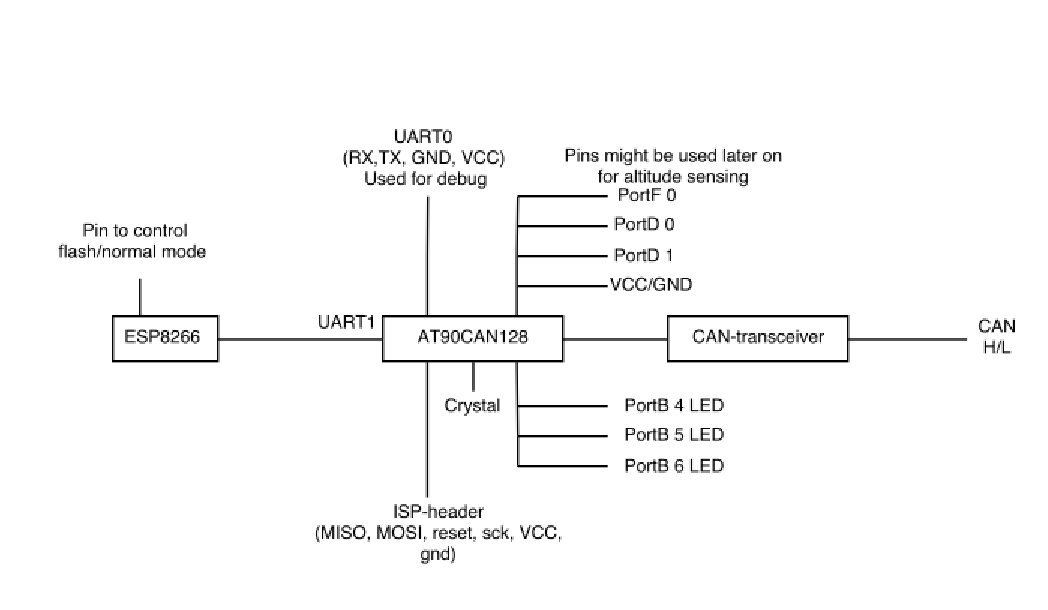
\includegraphics[width=1\textwidth]{graphics/PCB_block_v3.eps}
    \caption{Block schematic of the WIFI-extentionboard developed to AQ M4}
    \label{fig:PCB_block}
\end{figure}

\subsubsection{ATmega}
\subsubsection{Wireless Communication}
An important part of the hardware is the wireless communication used between the PC and the drones.
The wireless communication mpodule has severel requirements it needs to fulfill in order to make the whole system work as expected. A comparesiontable has been made in table \ref{tab:compare_table_wireless_communication} to find the wireless communication module that is best suited for the task.


\begin{table}[H]
	\centering
	\begin{tabular}{@{}|l|l|l|l|l|l|l|@{}}
		\toprule
		\textbf{Product} & \textbf{Size} & \textbf{Price} & 				\textbf{Usability} & \textbf{Power consumption} & 					\textbf{Range} & \textbf{Score} \\ \midrule
		ESP8266          &               &                &                    		&                            &                &                		\\ \midrule
		EMW3165          &               &                &                    		&                            &                &                		\\ \midrule
		nRF51822         &               &                &                    		&                            &                &                		\\ \bottomrule
	\end{tabular}
	\caption{Comparisontable used to compare different wireless 		communication modules}
	\label{tab:compare_table_wireless_communication}
\end{table}

\subsubsection{Pins}
A few pins where made available through solder pads for easy access if needed later on.

The following pins where available as solder pads:
\begin{itemize}
	\item PortF 0 - Alternative function as ADC, channel 0
	\item PortD 0 - Alternative function as interrupt, INT0
	\item PortD 1 - Alternative function as interrupt, INT1
\end{itemize}
In case the onboard baromter isn't accurate enough, an alternative distance could be used to measure the drones altitude with respect to the ground.
PortF0 has been made available since some distance sensors give output as an analogue value. 
An example of such sensor is an Infrared proximity sensor.\footnote{http://www.sharpsma.com/webfm\_send/1208} \\
As an alternative type of distance sensor, a ultrasoinc could be used such as HCSR04.
As output it gives a binary output with high-time proportional with the distance.\footnote{http://www.micropik.com/PDF/HCSR04.pdf}.
To detect the high-time, one of PortD1/0 would be useful. \\

Which type of sensor suits best as a distance sensor to provice altitude information to the drone is ouf of the scope of this report. The PCB has just been made ready to different types of sensors.

\subsubsection{Debug/ISP}
In the final schematic UART0 and ISP pins where combined in one pinheader for easy access through one cable. \Mathias{Refer to image of board}
To program the AtMega the ISP pins where required to be easy accessable. 
UART0 was made accessable to be used as debug and programming of the ESP8266 board.
The plan was to setup the AtMega as UART passthrough from UART0 to UART1.
Due to a mistake\footnote{The wrong pair of MISO/MOSI pins where made available in the ISP-header. The correct pair of MISO/MOSI is also RXD0/TXD0 as alternative function} in the final schematic, both UART0 and UART1 where made accessable trough the ISP/debug header. 
This ended up making it easier to program the ESP8266-board without using the AtMega as UART passthrough.



\chapter{Computer Vision in an Embedded System}\label{chp:VIS}
\input{vision}


\chapter{Communication between the UR5 and the EVS}\label{chp:COM}
\input{communication}

\chapter{Implementation of the EVS on the UR5}\label{chp:FinalImplementation}
\input{UR5_controller_system}

\chapter{Discussion and Conclusion}\label{chp:Conclusion}
\input{conclusion}
\chapter{Future Work}\label{chp:futurework}
\begin{itemize}
	\item Autodetect drones using avahi/mDNS. Instead of specificing the ID and ipaddress of each drone in the launch file, it could be handled automatically by avahi.
\end{itemize}


% --------- End Matter --------- %

\newpage
\listoffigures
%\begingroup
%\let\clearpage\relax
\newpage
\listoftables
%\endgroup

\begin{appendices}
\makeatletter
\addtocontents{toc}{\let\protect\l@chapter\protect\l@section}
\makeatother
\makeatletter
\addtocontents{toc}{\let\protect\l@section\protect\l@subsection}
\makeatother
\addtocontents{toc}{\protect\setcounter{tocdepth}{1}} % Exclude everthing from \section and downwards from ToC
\captionsetup{list=no} % Exclude all figures and tables from LoF and LoT

% Chapter 2 Hardware:
% Chapter 3 Vision:
\input{app_camera_calibration}
%\input{app_evs_object_detection}
\input{app_distance_calculation}
\input{app_opencv_functions}
\input{app_canny_edge}

% Chapter 4 Communication:
\input{app_dual_rpi_speed}
\input{app_K827P_speed}

% Chapter 5 UR5 Controller System:
%\input{app_final_implementation_benchmark}


\end{appendices}

%\bibliographystyle{siam}
%\bibliography{bibliography}
\printbibliography

\end{document}
